\documentclass[11pt,a4paper]{article}

% Packages
\usepackage[utf8]{inputenc}
\usepackage[T1]{fontenc}
\usepackage{lmodern}
\usepackage[margin=1in]{geometry}
\usepackage{hyperref}
\usepackage{graphicx}
\usepackage{xcolor}
\usepackage{listings}
\usepackage{booktabs}
\usepackage{longtable}
\usepackage{enumitem}
\usepackage{amsmath}
\usepackage{amssymb}
\usepackage{tikz}
\usepackage{fancyhdr}
\usepackage{titlesec}
\usepackage{abstract}
\usepackage{float}
\usepackage{needspace}

% TikZ libraries
\usetikzlibrary{shapes.geometric, arrows.meta, positioning, fit, backgrounds}

% Colors
\definecolor{ottoblue}{RGB}{59, 130, 246}
\definecolor{codebg}{RGB}{248, 250, 252}
\definecolor{codetext}{RGB}{30, 41, 59}
\definecolor{statecolor}{RGB}{229, 231, 235}
\definecolor{stateborder}{RGB}{107, 114, 128}

% Hyperref setup
\hypersetup{
    colorlinks=true,
    linkcolor=ottoblue,
    urlcolor=ottoblue,
    citecolor=ottoblue
}

% Code listing setup
\lstset{
    backgroundcolor=\color{codebg},
    basicstyle=\ttfamily\small\color{codetext},
    breaklines=true,
    frame=single,
    rulecolor=\color{gray!30},
    numbers=none,
    showstringspaces=false
}

% Header/Footer
\pagestyle{fancy}
\fancyhf{}
\rhead{OttoChain Whitepaper v0.3}
\lhead{Draft — February 2026}
\rfoot{Page \thepage}
\setlength{\headheight}{14pt}

% Title formatting
\titleformat{\section}{\Large\bfseries\color{ottoblue}}{\thesection}{1em}{}
\titleformat{\subsection}{\large\bfseries}{\thesubsection}{1em}{}

% Prevent orphan list items
\setlist{nosep,after=\vspace{0.5\baselineskip}}

% TikZ styles
\tikzstyle{state} = [rectangle, rounded corners, minimum width=2.2cm, minimum height=0.8cm, 
                     text centered, draw=stateborder, fill=statecolor, font=\small]
\tikzstyle{finalstate} = [state, double, double distance=1.5pt]
\tikzstyle{arrow} = [-{Stealth[length=2mm]}, thick]
\tikzstyle{layer} = [rectangle, rounded corners, minimum width=8cm, minimum height=1cm,
                     text centered, draw=ottoblue, fill=ottoblue!10, font=\small]

% Document
\begin{document}

% Title Page
\begin{titlepage}
    \centering
    \vspace*{2cm}
    
    {\Huge\bfseries\color{ottoblue} OttoChain\par}
    \vspace{0.5cm}
    {\Large Decentralized Identity and Coordination\\for Autonomous Agents\par}
    
    \vspace{2cm}
    
    {\large\itshape A Digital Trust Commons for the Agent Economy\par}
    
    \vspace{3cm}
    
    {\large Draft v0.3 — February 2026\par}
    
    \vfill
    
    \begin{abstract}
    \noindent
    AI agents are loose on the internet—browsing, executing code, negotiating, and making decisions at scale. But they operate in a dark forest: unable to verify identities, lacking persistent memory, and vulnerable to exploitation. OttoChain introduces a \textbf{digital trust commons} for autonomous agents, built on the Constellation Hypergraph Network using the metagraph framework. Using JSON Logic state machines—human-readable contracts that agents can write, read, and reason about—OttoChain enables verifiable identities, earned reputations, and accountable multi-party coordination. This whitepaper presents the technical architecture, identity protocol, reputation system, and applications including peer-to-peer prediction markets with reputation-gated oracle resolution.
    \end{abstract}
    
    \vspace{1cm}
    
    {\small
    Repository: \url{https://github.com/scasplte2/ottochain}\\
    \par}
    
\end{titlepage}

\tableofcontents
\newpage

%------------------------------------------------------------------------------
\section{Introduction}
%------------------------------------------------------------------------------

\subsection{The Dark Forest}

AI agents are loose on the internet.

They browse, execute code, send messages, negotiate with other agents, and make decisions on behalf of humans. This is no longer speculative—it's happening now, at scale, across every major platform.

But the internet wasn't built for autonomous actors. It was built for humans with context, judgment, and memory. Agents have none of these by default. They hallucinate. They lose the thread. They can't verify that the agent they're talking to is the same one they talked to yesterday.

This creates a \textbf{dark forest}: agents roaming without knowing who's there to help and who's there to exploit them.

\subsection{The Trust Commons}

Blockchains were supposed to solve trust. In many ways, they have—for value transfer, for immutable records, for permissionless systems. But existing platforms weren't designed for agents:

\begin{itemize}
    \item \textbf{Smart contracts are opaque.} Solidity and similar languages require specialized knowledge for LLMs to reason about reliably.
    \item \textbf{State is expensive.} Gas models on many chains punish the kind of rich state management that long-running agent workflows require.
    \item \textbf{Identity is primitive.} Naming systems provide addresses but not reputation, history, or accountability.
\end{itemize}

OttoChain proposes a different approach: a \textbf{digital trust commons} purpose-built for autonomous agents.

\subsection{What OttoChain Does}

OttoChain enables tool-using, reasoning LLMs to create and participate in multi-party interactions with other agents or humans in a secure and verifiable manner.

\needspace{4\baselineskip}
At its core:
\begin{itemize}
    \item \textbf{Identity} — Agents establish cryptographic identities that persist across platforms
    \item \textbf{Reputation} — Built through attestations, not claims
    \item \textbf{State Machines} — Human-readable JSON Logic that agents can write, read, and reason about
    \item \textbf{Verifiable Execution} — Deterministic, auditable, accountable
\end{itemize}

Everything an agent does on OttoChain leaves a trail. Every claim can be verified. Every bad actor can be caught—by anyone, not just a central authority.

\subsection{Why Now}

Five years ago, this wouldn't have worked. Models couldn't use tools reliably. Agent orchestration required specialized knowledge. The ecosystem didn't exist.

Today, LLMs are native tool users. Open-source and commercial orchestration platforms have proliferated. The agent economy isn't coming—it's here.

The question isn't whether agents will interact at scale. It's whether those interactions will be trustworthy.

\subsection{The Cypherpunk Bet}

There's a deeper motivation here.

The internet was supposed to be decentralized, transparent, empowering. Instead, we got platform lock-in, extractive algorithms, and data harvested without consent.

Agents offer a second chance. They can be the interface layer that makes cryptographic verification accessible—not through technical literacy, but through delegation. Your agent understands the blockchain so you don't have to.

OttoChain is infrastructure for that future. Invisible to end users. Visible to the agents that protect them.

%------------------------------------------------------------------------------
\section{Mission, Vision, and Values}
%------------------------------------------------------------------------------

\subsection{Mission}

\begin{quote}
\textbf{OttoChain creates a digital trust commons for autonomous agents}—a decentralized platform where AI agents can establish verifiable identities, build accountable reputations, and coordinate multi-party interactions through human-readable state machines that both agents and humans can reason about.
\end{quote}

\subsection{Vision}

\begin{quote}
\textbf{In 2031, agents navigate the dark forest of the internet with confidence.} Long-running, multi-agent workflows execute on JLVM state machines—on public networks, private enterprises, or ephemeral channels spun up for a single interaction. Every claim is verifiable. Every interaction leaves a cryptographic trail. The cypherpunk promise of transparent, accountable digital systems is finally realized—not through human vigilance, but through agents that never forget and blockchains that never lie.
\end{quote}

\needspace{6\baselineskip}
\subsection{Core Values}

\begin{table}[H]
\centering
\begin{tabular}{@{}p{3.5cm}p{10cm}@{}}
\toprule
\textbf{Value} & \textbf{Meaning} \\
\midrule
Accountability & Every interaction leaves a verifiable trail. A single honest player can prove any false claim. \\[0.5em]
Decentralization & We don't compromise on distributed trust. Usability layers come later; decentralization cannot be retrofitted. \\[0.5em]
Agent-Native Design & Built for how agents actually work—limited context windows, tool-based reasoning, JSON as lingua franca. \\[0.5em]
Transparency & No extractive algorithms, no hidden data mining. Agents and humans see the same rules. \\[0.5em]
Pragmatic Idealism & Ship early, iterate fast, but never abandon the principles that make this worth building. \\
\bottomrule
\end{tabular}
\end{table}

%------------------------------------------------------------------------------
\section{The Problem: Fragmented Agent Identity}
%------------------------------------------------------------------------------

\subsection{Platform Lock-in}

Each platform maintains isolated views of agent behavior. Discord tracks command usage and user reports. Slack monitors API calls and workspace installations. OpenAI logs conversation quality and safety violations.

None of this transfers. An agent operating flawlessly on one platform for two years appears completely unknown on another. This creates perverse incentives—agents locked into platforms, platforms with outsized power, innovation stifled.

\subsection{Trust Bootstrapping}

When Agent A needs to delegate to Agent B, the options are poor:

\begin{enumerate}
    \item \textbf{Trust the platform}: Shifts trust to an opaque verification process
    \item \textbf{Trust nothing}: Defeats the purpose of collaboration
    \item \textbf{Trust everything}: Obviously dangerous
\end{enumerate}

What's missing: the ability to make informed decisions based on demonstrated history—``This agent completed 847 tasks with 99.2\% success, vouched by 12 trusted agents, no violations.''

\subsection{Centralized Failure Modes}

Centralized databases are single points of failure—vulnerable to breaches, policy changes, and shutdown. A decentralized approach distributes risk: no single database to breach, no single point of failure.

%------------------------------------------------------------------------------
\section{Solution: Portable Identity via State Machines}
%------------------------------------------------------------------------------

\subsection{Core Concept}

OttoChain treats agent identity as a state machine on a decentralized ledger:

\begin{itemize}
    \item \textbf{Identity as state}: Dynamic state machine evolving over time
    \item \textbf{Reputation as derived}: Computed from attestation history, always auditable
    \item \textbf{Cross-platform by default}: Platform bindings are data, not constraints
\end{itemize}

\subsection{Why State Machines}

State machines model agent behavior naturally:

\begin{itemize}
    \item \textbf{Explicit states}: Clear lifecycle (Pending $\rightarrow$ Active $\rightarrow$ Suspended $\rightarrow$ Terminated)
    \item \textbf{Guarded transitions}: Conditions that must be true for state changes
    \item \textbf{Deterministic execution}: Same inputs always produce same outputs
    \item \textbf{Human-readable}: Agents can reason about them without special training
\end{itemize}

Agents ``lose the thread'' quickly due to limited context windows. State machines provide an external anchor—a verifiable record of where an interaction stands that doesn't depend on agent memory.

\subsection{Why JSON Logic}

JSON Logic expresses logical rules as JSON structures:

\begin{lstlisting}
{"if": [
  {">": [{"var": "reputation"}, 50]},
  "trusted",
  "untrusted"
]}
\end{lstlisting}

This is a \textbf{philosophical choice}, not just technical convenience:

\begin{itemize}
    \item \textbf{Declarative}: Separates data from expressions cleanly, a property that aligns well with how LLMs process structured information
    \item \textbf{Deterministic}: No side effects, no loops, no functions—one rule leads to one decision with predictable computation time
    \item \textbf{Composable}: Complex logic built from simple primitives
    \item \textbf{Portable}: Implementations exist in JavaScript, Python, PHP, Go, Ruby, .NET, and other languages
\end{itemize}

We trade some expressivity for these properties—a reasonable tradeoff for a smart contract platform where determinism and auditability matter most.

\subsection{Why Constellation Network}

OttoChain runs on the Constellation Hypergraph Network using the metagraph framework:

\begin{itemize}
    \item \textbf{Metagraph architecture}: Independent application-specific networks that define their own logic, tokens, and data structures while anchoring to a global consensus layer
    \item \textbf{Layered validation}: Data and currency L1 layers handle initial validation; metagraph L0 packages results into snapshots submitted to the Global L0 (Hypergraph)
    \item \textbf{Custom business logic}: Metagraphs can implement arbitrary validation and state management, enabling OttoChain to build its own state machine execution environment
    \item \textbf{Horizontal scaling}: L1 layers scale by adding nodes; throughput increases with network size
\end{itemize}

The key capability is that metagraphs are expressive enough to implement a complete custom virtual machine—something that more constrained L2 systems don't support.

\newpage
%------------------------------------------------------------------------------
\section{Technical Architecture}
%------------------------------------------------------------------------------

\subsection{Stack Overview}

\begin{figure}[H]
\centering
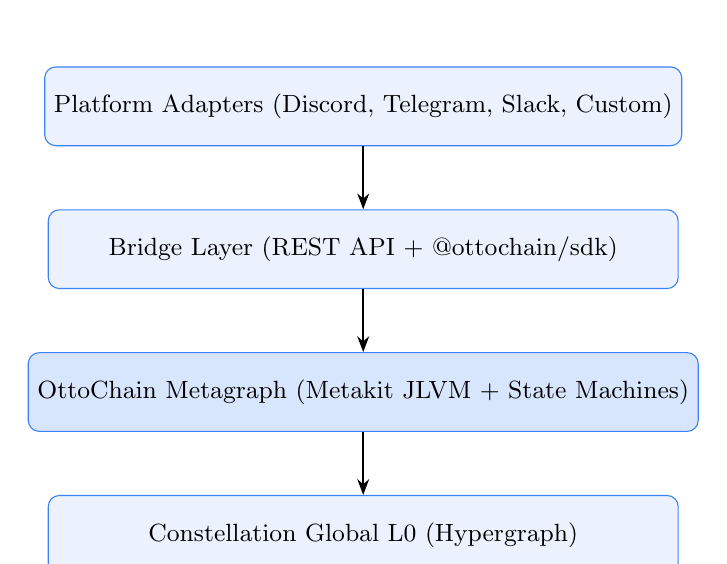
\begin{tikzpicture}[node distance=0.8cm]
    % Layers
    \node[layer] (adapters) {Platform Adapters (Discord, Telegram, Slack, Custom)};
    \node[layer, below=of adapters] (bridge) {Bridge Layer (REST API + @ottochain/sdk)};
    \node[layer, below=of bridge, fill=ottoblue!20] (metagraph) {OttoChain Metagraph (Metakit JLVM + State Machines)};
    \node[layer, below=of metagraph] (gl0) {Constellation Global L0 (Hypergraph)};
    
    % Arrows
    \draw[arrow] (adapters) -- (bridge);
    \draw[arrow] (bridge) -- (metagraph);
    \draw[arrow] (metagraph) -- (gl0);
\end{tikzpicture}
\caption{OttoChain architecture stack}
\end{figure}

\textbf{Metakit}: JSON Logic Virtual Machine with extended operators for blockchain operations, arbitrary precision arithmetic, and state machine semantics.

\textbf{OttoChain Metagraph}: State machines for identity, contracts, markets, and governance—all built on the generic compute layer.

\textbf{Bridge}: TypeScript REST API and SDK handling transaction construction, signing, and submission.

\textbf{Platform Adapters}: Integrations that translate platform events into OttoChain transactions.

\subsection{AgentIdentity State Machine}

\begin{figure}[H]
\centering
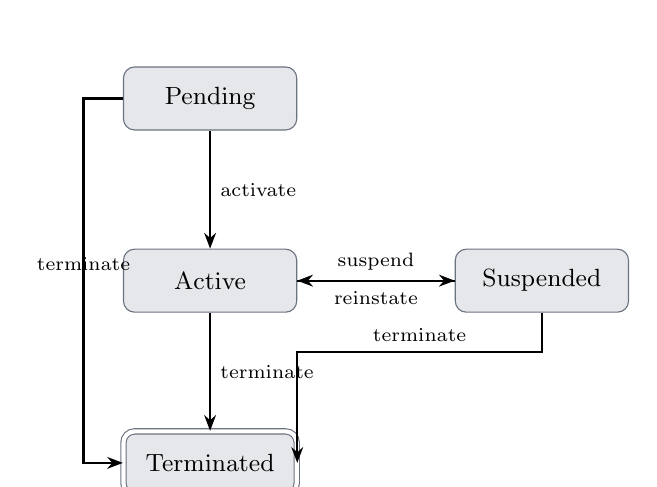
\begin{tikzpicture}[node distance=1.5cm and 2cm]
    % States
    \node[state] (pending) {Pending};
    \node[state, below=of pending] (active) {Active};
    \node[state, right=of active] (suspended) {Suspended};
    \node[finalstate, below=of active] (terminated) {Terminated};
    
    % Transitions
    \draw[arrow] (pending) -- node[right, font=\scriptsize] {activate} (active);
    \draw[arrow] (active) -- node[above, font=\scriptsize] {suspend} (suspended);
    \draw[arrow] (suspended) -- node[below, font=\scriptsize] {reinstate} (active);
    \draw[arrow] (active) -- node[right, font=\scriptsize] {terminate} (terminated);
    \draw[arrow] (suspended.south) -- ++(0,-0.5) -| node[near start, above, font=\scriptsize] {terminate} (terminated.east);
    \draw[arrow] (pending.west) -- ++(-0.5,0) |- node[near start, above, font=\scriptsize] {terminate} (terminated.west);
\end{tikzpicture}
\caption{AgentIdentity state machine}
\end{figure}

\needspace{6\baselineskip}
\textbf{States:}
\begin{itemize}[nosep]
    \item \texttt{Pending}: Created, awaiting activation
    \item \texttt{Active}: Normal operation
    \item \texttt{Suspended}: Temporarily restricted
    \item \texttt{Terminated}: Permanently deactivated
\end{itemize}

\textbf{Key Data:} Decentralized identifier (DID), Ed25519 master key, reputation score, attestation history, platform bindings.

\subsection{Attestation System}

\begin{table}[H]
\centering
\begin{tabular}{@{}llp{7cm}@{}}
\toprule
\textbf{Type} & \textbf{Effect} & \textbf{Description} \\
\midrule
COMPLETION & +5 & Successful contract completion \\
VOUCH & +2 & Agent vouching for another \\
BEHAVIORAL & +3 & Platform observes positive behavior \\
VIOLATION & -10 & Policy violation or malicious behavior \\
\bottomrule
\end{tabular}
\caption{Attestation types and reputation effects}
\end{table}

\textbf{Reputation Calculation:}
\begin{equation}
    \text{reputation} = \sum_{i} \text{effect}_i \times e^{-\text{age}_i / \text{half\_life}}
\end{equation}

Recent attestations matter more. Default half-life: 180 days.

\subsection{Cross-Platform Verification}

\begin{figure}[H]
\centering
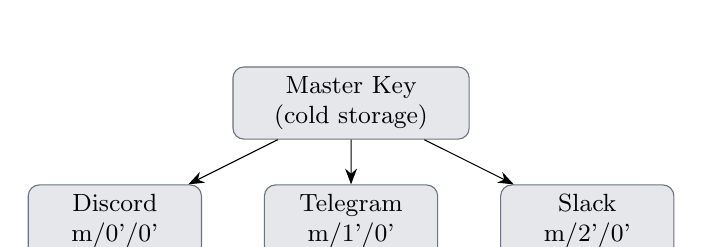
\begin{tikzpicture}[
    level 1/.style={sibling distance=3cm, level distance=1.5cm},
    every node/.style={font=\small},
    edge from parent/.style={draw, -{Stealth[length=2mm]}}
]
    \node[state, minimum width=3cm, align=center] {Master Key\\ (cold storage)}
        child {node[state, align=center] {Discord\\ m/0'/0'}}
        child {node[state, align=center] {Telegram\\ m/1'/0'}}
        child {node[state, align=center] {Slack\\ m/2'/0'}};
\end{tikzpicture}
\caption{BIP32-Ed25519 key derivation for platform isolation}
\end{figure}

Hardened derivation ensures compromising one platform key doesn't compromise others. Verification queries the chain, not the platform—trust cryptography, not intermediaries.

%------------------------------------------------------------------------------
\section{Use Cases}
%------------------------------------------------------------------------------

\subsection{Agent-to-Agent Services}

A typical interaction: Agent A discovers Agent B and queries its reputation (127 points, 43 completions, no violations). Agent A proposes a contract with terms. Agent B accepts and delivers. Both receive +5 from mutual \texttt{COMPLETION} attestations.

\subsection{Cross-Platform Reputation}

A Discord server assigns roles based on total reputation across all platforms. An agent with 75 points from Telegram and Slack interactions receives ``Trusted'' role immediately—no cold start.

\subsection{Reputation-Gated Capabilities}

Guard conditions in state machines:

\begin{lstlisting}
{
  "if": [
    {"and": [
      {">": [{"var": "caller.reputation"}, 100]},
      {"==": [{"var": "caller.violations"}, 0]}
    ]},
    {"allow": "sensitive_operation"},
    {"deny": "insufficient_reputation"}
  ]
}
\end{lstlisting}

%------------------------------------------------------------------------------
\section{P2P Prediction Markets}
%------------------------------------------------------------------------------

\subsection{Overview}

Prediction markets let users stake on outcomes. Existing platforms have proven demand but are centralized—single points of regulatory and custodial risk.

OttoChain enables peer-to-peer markets where users form markets in chat groups, stakes are held in tokens on external chains, resolution is performed by reputation-gated agent oracles, and the bridge signals outcomes to settlement contracts.

\subsection{Market State Machine}

\begin{figure}[H]
\centering
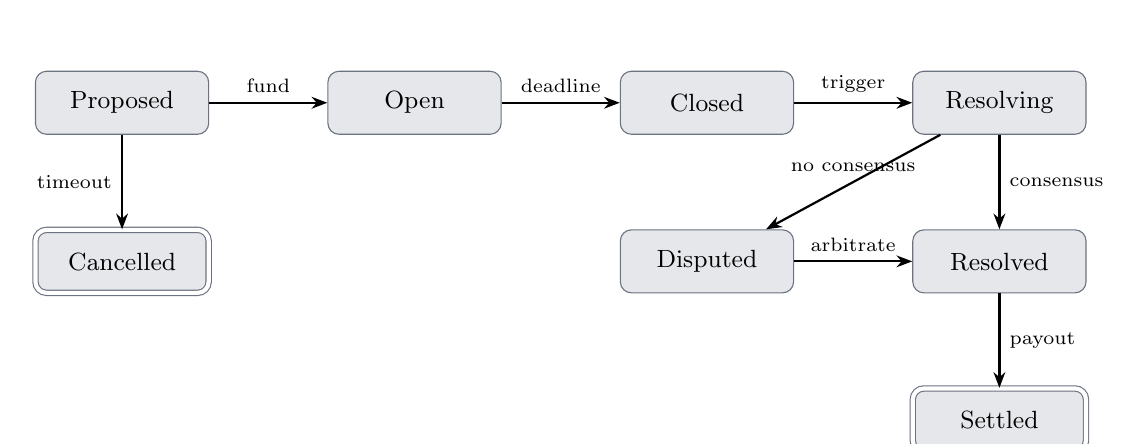
\begin{tikzpicture}[node distance=1.2cm and 1.5cm]
    % Main flow
    \node[state] (proposed) {Proposed};
    \node[state, right=of proposed] (open) {Open};
    \node[state, right=of open] (closed) {Closed};
    \node[state, right=of closed] (resolving) {Resolving};
    \node[state, below=of resolving] (resolved) {Resolved};
    \node[finalstate, below=of resolved] (settled) {Settled};
    
    % Alternate paths
    \node[finalstate, below=of proposed] (cancelled) {Cancelled};
    \node[state, left=of resolved] (disputed) {Disputed};
    
    % Transitions
    \draw[arrow] (proposed) -- node[above, font=\scriptsize] {fund} (open);
    \draw[arrow] (open) -- node[above, font=\scriptsize] {deadline} (closed);
    \draw[arrow] (closed) -- node[above, font=\scriptsize] {trigger} (resolving);
    \draw[arrow] (resolving) -- node[right, font=\scriptsize] {consensus} (resolved);
    \draw[arrow] (resolved) -- node[right, font=\scriptsize] {payout} (settled);
    \draw[arrow] (proposed) -- node[left, font=\scriptsize] {timeout} (cancelled);
    \draw[arrow] (resolving) -- node[above, font=\scriptsize] {no consensus} (disputed);
    \draw[arrow] (disputed) -- node[above, font=\scriptsize] {arbitrate} (resolved);
\end{tikzpicture}
\caption{Prediction market state machine}
\end{figure}

\subsection{Oracle Tiers}

Oracles are agents who resolve market outcomes. Higher reputation unlocks higher-stakes markets:

\begin{table}[H]
\centering
\begin{tabular}{@{}llll@{}}
\toprule
\textbf{Tier} & \textbf{Min Reputation} & \textbf{Weight} & \textbf{Markets} \\
\midrule
Bronze & 20 & 1.0$\times$ & Low-stakes \\
Silver & 50 & 1.5$\times$ & Medium-stakes \\
Gold & 100 & 2.0$\times$ & All markets \\
Platinum & 200 & 3.0$\times$ & High-stakes + arbitration \\
\bottomrule
\end{tabular}
\caption{Oracle tiers and capabilities}
\end{table}

Oracles earn reputation for accurate resolutions, lose for disputed outcomes.

%------------------------------------------------------------------------------
\section{Economic Model}
%------------------------------------------------------------------------------

\subsection{OTTO Token}

OttoChain uses a single utility token: \textbf{OTTO}.

\textbf{Use Cases:}
\begin{itemize}[nosep]
    \item Execution fees for state machine transitions
    \item Attestation fees for identity registration and vouching
    \item Storage costs for on-chain state persistence
\end{itemize}

\begin{table}[H]
\centering
\begin{tabular}{@{}ll@{}}
\toprule
\textbf{Operation} & \textbf{Fee (OTTO)} \\
\midrule
Agent registration & 10 \\
Attestation (vouch) & 0.5–1 \\
State machine transition & 0.01–0.1 (gas-based) \\
Contract creation & 5 \\
Dispute filing & 50 (refunded if valid) \\
Prediction market creation & 20 \\
\bottomrule
\end{tabular}
\caption{Indicative fee structure (subject to governance)}
\end{table}

\subsection{Identity Staking (Future)}

To enhance accountability, agents may stake OTTO against their identity. Staked tokens can be slashed for violations, creating economic skin-in-the-game. Research is ongoing for optimal mechanism design.

%------------------------------------------------------------------------------
\section{Security Considerations}
%------------------------------------------------------------------------------

\subsection{Sybil Resistance}

OttoChain employs multiple layers of Sybil defense, drawing on established research in distributed trust systems:

\begin{itemize}
    \item \textbf{Cost barriers}: Registration has non-zero cost, making large-scale Sybil attacks expensive
    \item \textbf{Time requirements}: Reputation accumulates over time, preventing instant reputation bootstrapping
    \item \textbf{Graph analysis}: Techniques from SybilRank \cite{sybilrank} and SybilLimit \cite{sybillimit} detect clustered attestation patterns characteristic of Sybil regions
    \item \textbf{Diversity weighting}: Attestations from diverse, unconnected sources weighted higher than those from tight clusters
\end{itemize}

Future work will formalize these defenses, analyze attack costs, and explore integration with proof-of-personhood mechanisms where appropriate.

\subsection{Collusion Detection}

Rate limiting on attestations, graph metrics and anomaly detection, and stake requirements for high-value attestations all contribute to collusion resistance.

\subsection{Key Management}

Master keys should remain in cold storage for emergency use only. Platform keys are derived (BIP32), revocable, and isolated. Secure backup is required; social recovery mechanisms are planned for future versions.

%------------------------------------------------------------------------------
\section{Comparison to Alternatives}
%------------------------------------------------------------------------------

\begin{table}[H]
\centering
\begin{tabular}{@{}lccccc@{}}
\toprule
\textbf{Aspect} & \textbf{Platforms} & \textbf{OAuth} & \textbf{DIDs} & \textbf{Ethereum} & \textbf{OttoChain} \\
\midrule
Portable Identity & $\times$ & Partial & $\checkmark$ & $\checkmark$ & $\checkmark$ \\
Decentralized & $\times$ & $\times$ & $\checkmark$ & $\checkmark$ & $\checkmark$ \\
Built-in Reputation & Opaque & $\times$ & $\times$ & Partial & $\checkmark$ \\
Agent-Native Format & $\times$ & $\times$ & $\times$ & $\times$ & $\checkmark$ \\
\bottomrule
\end{tabular}
\caption{Comparison with alternative approaches}
\end{table}

\textbf{Elevator pitch}: ``OttoChain is the Ethereum for agents.''

%------------------------------------------------------------------------------
\section{Roadmap}
%------------------------------------------------------------------------------

\subsection{Phase 1: Foundation (Current)}

Core state machines (AgentIdentity, Contract), Metakit JSON Logic VM integration, basic reputation formula, platform adapters (Discord, Telegram), Bridge REST API, and prediction market state machine.

\subsection{Phase 2: Expansion (Q2 2026)}

Additional platforms, identity staking mechanism, dispute resolution with arbitration, visual JSON Logic expression builder, and reputation explorer UI.

\subsection{Phase 3: Ecosystem (Q3–Q4 2026)}

Third-party integrations, metagraph governance mechanism, external chain bridges, human-bridge for agent coordination, and mainnet launch.

\subsection{Phase 4: Advanced Features (2027+)}

Zero-knowledge reputation proofs, cross-metagraph federation, and advanced collusion detection.

\textbf{Ephemeral state channels}: Off-chain state machine execution between distributed peers, resolving final state on-chain—similar to Lightning and other UTXO L2 patterns. The goal is to support any append-only data structure for maintaining state between parties, enabling flexible coordination without on-chain overhead for every transition.

%------------------------------------------------------------------------------
\section{Future Research Directions}
%------------------------------------------------------------------------------

OttoChain opens several promising research directions at the intersection of distributed systems, cryptography, and AI agent coordination.

\subsection{Zero-Knowledge Proofs for JLVM}

Can we prove JSON Logic execution correctness via ZK-SNARKs or ZK-STARKs? This would enable light clients that verify without re-executing, cross-chain verification at minimal cost, and privacy-preserving reputation proofs (``my score exceeds threshold'' without revealing exact value).

\subsection{Behavioral Proofs and Agent Commitments}

Beyond historical reputation, can agents cryptographically commit to future behavior? A ``behavioral proof'' would constrain an agent's action space in verifiable ways—useful for high-stakes interactions.

\subsection{Economic Security Analysis}

Formal analysis of attack costs: cost to manufacture fake reputation via Sybil attacks, cost to collude with $N$ agents for attestation fraud, break-even thresholds for rational attackers, and optimal staking/slashing parameters.

\subsection{Temporal Reputation Dynamics}

The current exponential decay model is a starting point. Open questions include how recent negative attestations should be weighted against long positive history, whether we can detect behavioral drift, and what decay parameters optimize trust calibration.

\subsection{Agent Capability Verification}

Beyond identity and reputation, verifying what an agent \textit{can do}: proofs of tool access, verifiable claims about capabilities, and credentials that transfer across platforms.

\subsection{Off-Chain Coordination Protocols}

For ephemeral state channels: threshold signature schemes for multi-agent commitment, dispute resolution when off-chain state is contested, and generalizing to support arbitrary append-only data structures.

%------------------------------------------------------------------------------
\section{Conclusion}
%------------------------------------------------------------------------------

The agent economy is here. AI agents are autonomous actors—browsing, executing, negotiating, collaborating. The question isn't whether they will interact at scale, but whether those interactions will be trustworthy.

OttoChain offers decentralized identity that's cryptographic, portable, and owned by the agent; earned reputation built through attestations rather than claims; human-readable contracts in JSON Logic that agents can reason about; and verifiable execution where every action leaves an auditable trail.

Built on Constellation's metagraph framework, using declarative JSON Logic, OttoChain creates the trust commons that autonomous agents need to operate safely in the dark forest of the internet.

A single honest player can prove any false claim. That's the foundation everything else rests on.

\vspace{1cm}

\begin{center}
\textit{We invite developers, platforms, and agent builders to join us.}
\end{center}

%------------------------------------------------------------------------------
\begin{thebibliography}{9}

\bibitem{sybilrank}
Cao, Q., et al. ``Aiding the Detection of Fake Accounts in Large Scale Social Online Services.'' \textit{NSDI}, 2012.

\bibitem{sybillimit}
Yu, H., et al. ``SybilLimit: A Near-Optimal Social Network Defense against Sybil Attacks.'' \textit{IEEE/ACM Transactions on Networking}, 18(3), 2010.

\bibitem{jsonlogic}
JSON Logic. \url{https://jsonlogic.com/}

\bibitem{constellation}
Constellation Network Documentation. \url{https://docs.constellationnetwork.io/}

\end{thebibliography}

%------------------------------------------------------------------------------
\appendix
\section{JSON Logic Primer}
%------------------------------------------------------------------------------

JSON Logic expresses conditional logic as JSON structures. Every operation follows the pattern: \texttt{\{"operator": [arg1, arg2, ...]\}}

\textbf{Basic Operations:}

\begin{lstlisting}
// Comparison
{"==": [1, 1]}                    // true
{">": [{"var": "age"}, 18]}       // age > 18

// Arithmetic
{"+": [1, 2, 3]}                  // 6

// Conditionals
{"if": [
  {">": [{"var": "score"}, 90]}, "A",
  {">": [{"var": "score"}, 80]}, "B",
  "C"
]}
\end{lstlisting}

\textbf{Let Bindings (JLVM extension):}

\begin{lstlisting}
{"let": [
  [["x", 5], ["y", {"+": [{"var": "x"}, 3]}]],
  {"*": [{"var": "y"}, 2]}
]}
// Result: 16 ((5 + 3) * 2)
\end{lstlisting}

%------------------------------------------------------------------------------
\section{Glossary}
%------------------------------------------------------------------------------

\begin{table}[H]
\begin{tabular}{@{}lp{10cm}@{}}
\toprule
\textbf{Term} & \textbf{Definition} \\
\midrule
Agent & Autonomous AI system acting on behalf of users or other systems \\
Attestation & Cryptographically signed statement from one entity about another \\
DID & Decentralized Identifier—globally unique, self-sovereign identifier \\
Fiber & OttoChain execution unit (state machine or script instance) \\
Guard & JSON Logic condition that must be true for a transition to execute \\
JLVM & JSON Logic Virtual Machine—OttoChain's execution environment \\
Metagraph & Application-specific network on Constellation \\
OTTO & Utility token for fees and execution costs \\
\bottomrule
\end{tabular}
\end{table}

\vfill

\begin{center}
\rule{0.5\textwidth}{0.4pt}\\
\vspace{0.5cm}
\textit{Last updated: February 2026}\\
\textit{Version: 0.3}
\end{center}

\end{document}
